% THIS IS SIGPROC-SP.TEX - VERSION 3.0
% WORKS WITH V3.1SP OF ACM_PROC_ARTICLE-SP.CLS
% JUNE 2007
%
% It is an example file showing how to use the 'acm_proc_article-sp.cls' V3.1SP
% LaTeX2e document class file for Conference Proceedings submissions.
% ----------------------------------------------------------------------------------------------------------------
% This .tex file (and associated .cls V3.1SP) *DOES NOT* produce:
%       1) The Permission Statement
%       2) The Conference (location) Info information
%       3) The Copyright Line with ACM data
%       4) Page numbering
% ---------------------------------------------------------------------------------------------------------------
% It is an example which *does* use the .bib file (from which the .bbl file
% is produced).
% REMEMBER HOWEVER: After having produced the .bbl file,
% and prior to final submission,
% you need to 'insert'  your .bbl file into your source .tex file so as to provide
% ONE 'self-contained' source file.
%
% Questions regarding SIGS should be sent to
% Adrienne Griscti ---> griscti@acm.org
%
% Questions/suggestions regarding the guidelines, .tex and .cls files, etc. to
% Gerald Murray ---> murray@acm.org
%
% For tracking purposes - this is V3.0SP - JUNE 2007

\documentclass{acm_proc_article-sp}
\usepackage{listings}
\usepackage{url}
\usepackage{cite}

\lstset{numbers=left, columns=flexible, language=[AspectJ]Java, basicstyle=\small, numberstyle=\tiny, frame=tb}
\lstset{
morekeywords={own,module,export,as,merge,{module\_interface}, replace, with, overrides, singleton, supermodule},
frame=tb,
numbers=left,
captionpos=t,
tabsize=2
}

\begin{document}

\title{Extensible Inter-type Declarations Through Modules}
%
% You need the command \numberofauthors to handle the 'placement
% and alignment' of the authors beneath the title.
%
% For aesthetic reasons, we recommend 'three authors at a time'
% i.e. three 'name/affiliation blocks' be placed beneath the title.
%
% NOTE: You are NOT restricted in how many 'rows' of
% "name/affiliations" may appear. We just ask that you restrict
% the number of 'columns' to three.
%
% Because of the available 'opening page real-estate'
% we ask you to refrain from putting more than six authors
% (two rows with three columns) beneath the article title.
% More than six makes the first-page appear very cluttered indeed.
%
% Use the \alignauthor commands to handle the names
% and affiliations for an 'aesthetic maximum' of six authors.
% Add names, affiliations, addresses for
% the seventh etc. author(s) as the argument for the
% \additionalauthors command.
% These 'additional authors' will be output/set for you
% without further effort on your part as the last section in
% the body of your article BEFORE References or any Appendices.

\numberofauthors{2} %  in this sample file, there are a *total*
% of EIGHT authors. SIX appear on the 'first-page' (for formatting
% reasons) and the remaining two appear in the \additionalauthors section.
%
\author{
% You can go ahead and credit any number of authors here,
% e.g. one 'row of three' or two rows (consisting of one row of three
% and a second row of one, two or three).
%
% The command \alignauthor (no curly braces needed) should
% precede each author name, affiliation/snail-mail address and
% e-mail address. Additionally, tag each line of
% affiliation/address with \affaddr, and tag the
% e-mail address with \email.
%
% 1st. author
\alignauthor
Neil Ongkingco\\
       \affaddr{Programming Tools Group}\\
       \affaddr{University of Oxford}\\
       \email{neil.ongkingco@gmail.com}\\
% 2nd. author
\alignauthor
Torbj\"{o}rn Ekman\\
       \affaddr{Programming Tools Group}\\
       \affaddr{University of Oxford}\\
       \email{Torbjorn.Ekman@comlab.ox.ac.uk}\\
}
% There's nothing stopping you putting the seventh, eighth, etc.
% author on the opening page (as the 'third row') but we ask,
% for aesthetic reasons that you place these 'additional authors'
% in the \additional authors block, viz.

% Just remember to make sure that the TOTAL number of authors
% is the number that will appear on the first page PLUS the
% number that will appear in the \additionalauthors section.

\maketitle
\begin{abstract}

Inter-type declarations (ITDs) in current aspect-oriented languages have
limited extensibility: it is difficult to change the behavior of
existing ITDs when extending a system written in an aspect-oriented
language. We introduce a module system that allows for ITD extensibility 
through module subtyping, and demonstrate that modules also provide 
the additional benefits of information hiding and explicit dependency 
specification. The module system is also used on a moderately-sized 
case study on a Java compiler written in JastAdd, an aspect-oriented 
compiler construction framework.

\end{abstract}


%A category including the fourth, optional field follows...
\category{D.3.3}{Programming Languages}{Language Constructs and Features}

\terms{Languages, Design, Module}

\keywords{Modularity, Aspect-Oriented Programming, JastAdd} 

\section{Introduction}
\label{section:introduction}
Inter-type declarations (ITDs) provide a powerful yet simple modularization
mechanism. The possibility to extend existing classes modularly without
ahead-of-time planning is not only useful to separate different concerns
but also extremely convenient for modular extensibility when software
evolves.

A common criticism of ITDs is their global scope which arguably leads to
poor information hiding, a topic that has gained renewed interest with the 
emerging support for modules in Java 7. Another disadvantage is that the 
class hierarchy is destructively updated, preventing multiple variants of 
classes with different sets of ITDs applied. It is worth noting that 
this drawback is not shared by more traditional extension mechanisms such 
as visitors. The problem of how to handle multiple variants of the same 
class exist in plain Java as JAR hell, and there has been a wealth of work 
on module systems for Java-like languages to improve on status quo. We use 
this existing work on Java modules in an attempt to solve the class 
variant problem for ITDs.

The emerging support for modules in Java 7 enhances information hiding and
extended module proposals such as Strni\v{s}a gives hope for simultaneous
deployment of multiple versions of the same library in different modules.
Modules provide information hiding at a level higher than packages. Module
systems like OSGi bundles\cite{OSGi4} and the proposed Java module system\cite{JSR277}
allow the explicit definition of the dependencies of a module. We can extend
the information hiding features of these module systems to extend to aspects, 
so as to limit the scope of ITDs.
Another module system, iJAM \cite{iJAM}, adds explicit module instantiation, 
which allows multiple versions of the same module to coexist in a single compilation.
This is built upon by some of our previous work \cite{modulesastypes}, which 
adds the idea of treating modules as object-oriented types, with instantiation
similar to iJAM and additional operations to allow explicit and fine-grained
module instance sharing. 

%ITDs are global in their nature which makes local
%reasoning somewhat difficult, and as an extensibility mechanism they can be
%improved by enabling deployment of multiple versions of libraries, 
%each woven a with different set of ITDs.


Previous work show how aspects can be improved using modules for point-cut
and advice \cite{openmodulesaj}. Aspects don't work very well without 
modules, due to global scope and implicit dependencies. We believe that 
such benefits are even more important for a system with inter-type 
declarations. In this paper we therefore present a module system that 
supports inter-type declarations and improve their use when extending a 
system in a modular fashion.

%Aspect instantiation has always been a sticky subject (e.g. doubly applied
%pointcuts in AspectJ abstract aspects)

We have extended previous work on object-oriented modules for Java \cite{modulesastypes}, 
and implemented the proposed module system as an extension to the 
Jast\-Add system, an aspect oriented compiler construction system 
extending Java with support for attribute grammars and ITDs. That system is itself an extension 
to the Jast\-Add Extensible Java compiler (Jast\-AddJ), a Java frontend and compiler
which is used in for instance the AspectBench compiler for AspectJ, and the 
Soot bytecode manipulation framework. The implementation of ITDs in the JastAdd
system is actually shared with the implementation of ITDs in the
AspectBench Compiler for AspectJ. 

To evaluate the module system we performed a case study where JastAddJ was 
refactored to use the proposed module system. It is important to 
distinguish JastAdd, a meta compiler system used to build JastAddJ, from JastAddJ, a Java 
compiler, since both are used as examples in the paper.

In our previous work we explain how to use ITDs as one of the main
modularization mechanisms when building extensible compilers \cite{aosd08abc}. Our current
work involves using the same techniques to generate IDEs for a wide range
of dialects of Java. In such an IDE we may for instance want to use numerous variants of the
same frontend that slightly differ to support different dialects. We also
want to use a pure frontend for error checking while a backend is also
needed to support code generation.
That work highlights some deficiencies to ITDs from an extensibility point of
view compared to the more traditional use of visitors.
Inter-type declarations have the advantages of not requiring ahead-of-time 
planning, the ability to add state, no need for boiler-plate code, and 
being less error prone since adherence to framework 
conventions to enable dispatch is not necessary.
However, ITDs do not provide the same level of extensibility as visitors.
ITDs are currently destructive updates of the class hierarchy. The base version and the
extended version can not co-exist. This is the main motivation for our
work. 
Our case study shows that the proposed module system solves these deficiencies completely in an
elegant fashion, and also enhances information hiding by restricting 
visibility of large parts of the system that used to be globally visible.

These are the main contributions of this paper:
\begin{itemize}
\item The design of a module system for ITDs that improves information
hiding and extensibility.
\item An implementation as a modular extension to the Jast\-Add meta 
compiler system.
\item A case study where implementation of the Java compiler JastAddJ is retrofitted to use the
proposed module system.
\end{itemize}

The rest of this paper is structured as follows: In
Section~\ref{section:itdvisitors} we present a detailed example that
highlight the merits and deficiencies of ITDs compared to a visitor based
approach. A module system that shows how that example can be improved is
presented in Section~\ref{section:jastaddmodules} and we present a case
study where an extensible Java compiler is retrofitted to use that module
system in Section~\ref{section:casestudy} where we also discuss 
the advantages it brings compared to the original implementation. A
brief overview of the module system implementation is presented in
Section~\ref{section:implementation} and we discuss related work in
Section~\ref{section:related} and conclude in
Section~\ref{section:conclusions}.



\section{ITDs vs. Visitors}
\label{section:itdvisitors}
In this section we present two alternative implementations of a small
calculator, one using visitors and one using ITDs. It will be used as a
running example throughout the paper to illustrate the advantages and
disadvantages of the respective solution. In Section~\ref{section:jastaddmodules}
we then present a module system for ITDs that removes some of the presented
deficiencies.

\subsection{Running Example: Calculator}
Consider a tiny calculator supporting integer literals and addition, thus 
supporting composite expressions like: 1 + 2. It may seem trivial but its 
implementation illustrates some important extensibility challenges that we 
address in this paper. The calculator supports various computations on top 
of this structure, e.g., evaluating its value and printing its string
representation.

To evaluate the extensibility of a visitor based solution and an ITD based
solution we extend the calculator with two small extensions: first support
for subtraction and then support for an alternative string representation 
where constants are printed using natural language, i.e., one, two, 
three, etc.

%TODO: %Introduce the Expression problem.

Notice that this is a simplified example of a compiler. Information is
for instance only propagated bottom up so there is no need for parameter
propagation during a visit. Parameters would require a significantly more 
complex visitor due to the requirement on contravariance in the argument 
for type safety would require much more complex genericity. We chose an 
example that is flattering for visitors to be fair when arguing that ITDs 
are a more suitable solution even in this case. While the example is 
tiny the same structure is commonly used in compilers. In~\cite{aosd08abc} we argue 
the merits of using ITDs and attribute grammars rather than visitors in 
extensible compiler construction, using a complete Java compiler as a 
major case study.

\subsection{Visitor Implementation}
A visitor based solution uses the composite design pattern to model the
static structure of expressions: one class for each language element and
composition of language elements forming a tree structure. That is, the 
Add node has references to its left and right child respectively, while 
the Int node has a single filed holding its value.

Each node type also contains an accept method that performs an additional
dispatch to select the code in the visitor for the concrete node type. 
This double dispatch scheme is the key to dispatching both on the node 
type and the visitor. We can thus select a particular method that is
selected based on both the dynamic type of the receiving object and the 
dynamic type of the visitor, provided as a parameter. 

A visitor is then simply a class that holds an implementation for each concrete 
class type that may accept the visitor. The Eval visitor computes the 
value for Int and Add, while the Print visitor computes a string 
representation for each expression in a similar fashion. The visitor code 
is required to visit children indirectly using the accept method which 
clutters the implementation and is somewhat error prone.

\begin{lstlisting}[caption={Visitor Base}]
abstract class Expr {
  abstract <T> T accept(Visitor<T> v);
}
class Int extends Expr {
  int value;
  <T> T accept(Visitor<T> v) {
    return v.visitInt(this);
  }
}
class Add extends Expr {
  Expr left;
  Expr right;
  <T> accept(Visitor<T> v) {
    return v.visitAdd(this);
  }
}
class Visitor<T> {
  <T> visitInt(Int i) { return null; }
  <T> visitAdd(Add a) { return null; }
}

class Eval extends Visitor<Integer> {
  Integer visitInt(Int i) {
    return i.value;
  }
  Integer visitAdd(Add a) {
    return a.left.accept(this) + a.right.accept(this);
  }
}
class PrettyPrinter extends Visitor<String> {
  String visitInt(Int i) {
    return Integer.toString(i.value);
  }
  String visitAdd(Add a) {
    return a.left.accept(this) + " + " + a.right.accept(this);
  }
}
\end{lstlisting}

\subsection{ITD Implementation}
The ITD implementation of the calculator has a similar implementation of the
node types as the visitor based solution, but the accept methods are no
longer necessary. Instead the aspect Eval introduces an eval method in each
node type. These methods can then be called from other introduced methods
directly without the need for using accept methods to enable dispatch.

\begin{lstlisting}[caption={ITD Base}]
abstract class Expr {
}
class Int extends Expr {
  int value;
}
class Add extends Expr {
  Expr left;
  Expr right;
}
aspect Eval {
  abstract int Expr.eval();
  int Int.eval() {
    return value;
  }
  int Add.eval() {
    return left.eval() + right.eval();
  }
}
aspect PrettyPrinter {
  abstract String Expr.print();
  String Int.print() {
    return Integer.toString(value);
  }
  String Add.print() {
    return left.print() + " + " + right.print();
  }
}
\end{lstlisting}

\subsection{Extension}
As an example of extension we first add a subtraction node and enable the
existing analyses to support that new operation. Then, we add a new
analysis that computes a string representation of an expression where the
literals are printed using natural language.

\subsubsection{Visitor extension}
We need to add a new node type Sub that includes the boiler plate code to
support the visitor pattern. Then the base visitor is extended to support
the new node type. This change is not completely modular but a pragmatic
choice to keep the solution simple. We could have used various tricks with advanced
generics concepts, but that would make the solution even more complex and 
clutter the solution with framework code. It should be admitted that the 
current solution is not
completely safe since the default implementation for visitSub is not
suitable for the Eval and Print visitors. 

We also provide extended vistitors
,ExtEval and ExtPrint, to support the extended language.
They can extend the base behavior and simply provide the increment
needed to support the subtraction operation. The extended version of the
printer can then be refined to display integer constants using natural
language in the separate visitor WordPrint. Notice that functionality from
the base visitor can be reused here as well and only the functionality 
that is refined need to be provided.

\begin{lstlisting}[caption={Visitor Extension}]
class Sub extends Expr {
  Expr left;
  Expr right;
  T accept(Visitor<T> v) {
    return v.visitSub(this);
  }
}
class Visitor<T> { // replace old impl.
  T visitInt(Int i) { return null; }
  T visitAdd(Add a) { return null; }
  T visitSub(Sub s) { return null; } // new
}
class ExtEval extends Eval {
  Integer visitSub(Sub s) {
    return a.left.accept(this) - a.right.accept(this);
  }
}
class ExtPrint extends Print {
  String visitSub(Sub s) {
    return a.left.accept(this) + " - " + a.right.accept(this);
  }
}
class WordPrint extends ExtPrint {
  Integer visitInt(Int i) {
    .. convert i to the strings "one", "two", etc.
  }
}
\end{lstlisting}

\subsubsection{ITD extension}
The ITD-based solution simply adds a new node type and introduces methods in that
node type to make the evaluator and printer support subtraction.
The natural language based printer is slightly more complicated. The simple
model of introducing new methods in an existing class is not as convenient
in this case. We can not keep the implementation printing numbers and reuse
the other printing functionality while still changing it to print using
natural language. The word printer therefore choses to take precedence over
the other definitions of \texttt{print} making it the only implementation, thus
disabling the normal printer.

\begin{lstlisting}[caption={ITD Extension}]
class Sub extends Expr {
  Expr left;
  Expr right;
}
aspect ExtEval {
  int Sub.eval() {
    return left.eval() - right.eval();
  }
}
aspect ExtPrint {
  String Sub.print() {
    return left.print() + " - " + right.print(); 
  }
}
aspect WordPrint {
  declare precedence: WordPrint, *;
  String Int.print() {
    .. convert i to the strings "one", "two", etc.
  }
}
\end{lstlisting}

\subsection{Discussion}
While both presented solutions are quite similar there are some important
differences:

Visitors require some ahead of time planning with boiler plate code in the 
node types while the ITD solution can modularly update an existing class 
hierarchy if needed. The actual visitors can be updated in a 
modular fashion using inheritance and overriding but the user of these 
analyses need to update the code to use the extended versions. ITDs can 
be used to directly add support for existing analyses in the new node type 
in a completely modular fashion. 

The visitor based solution need to include framework code to enable the 
double dispatch pattern which clutters the implementation and is somewhat 
error prone. The ITD solution on the other hand is quite 
straightforward with a clean implementation.

The base visitor could not be modularly extended in the presented example.
There are solutions based on advanced usage of generics that support
modular extension but that requires much more framework code and clutters
the solution even more. Moreover, the user need still replace uses of the
old visitors with uses of the new visitor.

Visitors can be inherited and overridden to refine behavior in a visitor
being extended. This enables both visitors to be used in the same system
while the ITD solution can only use either the original implementation 
or the refined implementation. 

%%Removed for now, we don't address this issue in the module solution.
%Another advantage of the visitor based solution is that each class can be
%modularly type-checked and compiled while the ITD based solution requires a
%global analysis since methods can be introduced by any aspect in the
%system.


\section{Module System for ITDs}
\label{section:jastaddmodules}
The previous section has shown that while ITD implementations are generally
cleaner and require less ahead-of-time planning to allow extensibility, they
are still limited by their global scope: two versions of the same ITD cannot
exist in the same system. We now propose to remedy this problem by introducing
an aspect-aware module system that allows for multiple instances of classes
to exist, each instance modified by a particular version of the ITDs.

The module system is based on the object-oriented java module system 
presented in \textit{Modules as Object-Oriented Types}\cite{modulesastypes},
and the aspect-oriented features are provided by Jast\-Add\cite{jastadd, jastaddjavacompiler}, 
an aspect-oriented compiler framework. Jast\-Add uses the same ITD 
syntax as in AspectJ, and should therefore be familiar to the expected audience
of this paper.

\subsection{Module System Overview}

A module consists of aspects and classes, and defines the set of external
modules that are visible to the module's members. 
A module is considered to be the type of the collection of classes and aspects
that belong to it. The module system allows the instantiation these module types
within the context of an importing module, defines a subtyping relation
on module types, and a merge operation to manipulate module instances.

The remainder of this section goes into the details of the module system, and shows
how it can be used the enhance the ITD solution to the calculator 
presented in Section~\ref{section:itdvisitors}.

\subsection{Declaration and Membership}

A module is defined in a \texttt{.module} file, and is headed by the module's name:

\begin{lstlisting}[caption={Module Declaration}]
//file prettyprinter.module
module prettyprinter;
...
\end{lstlisting}

Membership to a module is defined in the compilation unit of the members,
similar to a package declaration:

\begin{lstlisting}[caption={Module Membership}]
//file Print.jrag
module prettyprinter; //module membership
public aspect Print {
	public abstract String Expr.print();
	
	public String Add.print() {
		return getLeft().print() + 
				"+" + getRight().print();
	}
	
	public String IntLit.print() {
		return getIntLit().toString();
	}
}

//file Expr.java
module asttypes; //module membership
package expr; //package declaration
public class Expr {
...
}
\end{lstlisting}

Module and package declarations can coexist in a single compilation unit.
Modules can contain aspects and classes that span multiple packages.

\subsection{Module Access Control}

Packages are not implicitly visible outside the module unless an
\texttt{export} declaration is provided for that package. These declarations
are placed in \texttt{.module} files.

\begin{lstlisting}[caption={Export Package}]
//file asttypes.module
module asttypes;
export package expr, stmt; //export expr and stmt
...

//file prettyprinter.module
module prettyprinter;
export package *; //export all packages
...
\end{lstlisting}

As the example shows, an export package may contain a list of packages, or the
wildcard \texttt{*}, which exposes all packages in the module. Any types that
belong to a package that is not exported are not visible from outside the module.

The module system also introduces the module-private access modifier \textbf{module},
which allows access to a type, method or field from the within the same module. This
allows more fine-grained control over the set of publicly accessible types of a module.

\begin{lstlisting}
//file Expr.java
module asttypes;
//only visible from module asttypes
module class Expr {
	//only visible from module asttypes
	module int moduleField;
	module void moduleMethod() {...}
}
\end{lstlisting}

\subsection{Imports and Instantiation}

Module definitions also contain import declarations, which specify which
other modules are visible to the members of the module. A module imports 
an \textit{instance} of another module, which allows multiple instances
of the same module to exist within a single context.

An import in a module declaration creates a typed module reference which is pointed to
an instance of that module type. 
There are two ways to import a module instance: importing the singleton or
an \textbf{own} instance. Imports may also be aliased to allow multiple instances
of the same module to exist in the same context, and be exported so that
they are also accessible through indirection from other modules.

\begin{lstlisting}[caption={Imports}, label={figure:imports}]
//file prettyprinter.module
module prettyprinter;
//import the singleton instance of module parserframework
import parserframework; 
//import an own instance of the module asttypes
import own asttype;
//import another instance of asttype, using an alias and export
import own asttype export as public_ast;
\end{lstlisting}

Imports of \textbf{own} instances without an explicit alias use the name
of the imported module as its alias. To be more specific, line 6 from the above
example is equivalent to
\begin{lstlisting}
import own asttype as asttype;
\end{lstlisting}

Import cycles involving \textbf{own} instances are not allowed as they
lead to infinite module instance creation. Import cycles involving only
singleton instances, however, are allowed.

An aspect can only introduce ITDs to types that are visible from its parent module. 
This allows the use of module imports and access modifiers to control dependencies
caused by ITDs.

Importing the singleton module allows different modules to share the same instance
of the same module type. This allows the sharing of classes across modules, as
classes that belong to different instances of a module are not type compatible.
In the presence of the \textbf{merge} operator (described later), a singleton import
also ensures that the imported module is an unmodified version of the base module type.

The visibility of imported modules become important for module qualifiers and the \textbf{merge} operation, described later.

\subsection{Module Qualified Type Accesses}

Allowing two instances of the same module to exist in the same context
requires a way to disambiguate references to the members of the instances.
We introduce \textit{module qualifiers} for type references to explicitly
choose the module to which the type belongs.

A module qualified type access takes this form:

\begin{lstlisting}
modulealias::packagename.TypeName
\end{lstlisting}

The following example uses the module definition from listing \ref{figure:imports}.
The module \texttt{prettyprinter} imports two instances of \texttt{asttype}, with the
aliases \texttt{asttype} and \texttt{public\_ast}. The aspect \texttt{Print},
which belongs to the module, introduces ITDs to each of the \texttt{Add} types
of the instances.

\begin{lstlisting}[caption={Module Qualifiers}]
//file Print.jrag
module prettyprinter;
aspect Print {
	...
	//modifies the Add type in asttypes
	public String asttypes::Add.print() {
		//infix print
		return getLeft().print() + "+" + 
				getRight().print();
	}
	...
	//modifies the Add type in public_ast
	public String public_ast::Add.print() {
		//postfix print
		return getLeft().print() + 
				getRight().print() + "+";
	}
}
\end{lstlisting}

Module qualifiers also allow for indirection. A module can be accessed 
through its importing module if it was exported. A type access
that uses module indirection takes the form:

\begin{lstlisting}
modulealias1::modulealias2::packagename.TypeName
\end{lstlisting}

The following example
shows a small system consisting of the modules \texttt{scanner}, 
\texttt{parser} and \texttt{parserapp}. The parser module imports
the scanner module, and the parser application module imports the
parser. The parser application module then adds an ITD to the classes
\texttt{Scanner} and \texttt{Parser}, which are members of the scanner
and parser modules respectively. The import statements in the 
\texttt{ParserApp.jrag} file in the example are normal java import
statements, to demonstrate that module qualifiers are also allowed
for that language construct.

\begin{lstlisting}
//file scanner.module
module scanner;
export package *;
...

//file parser.module
module parser;
//allow access to imported scanner
import own scanner export as scanner;
export package *;
...

//file parserapp.module
module parserapp;
import own parser;
...

//file ParserApp.jrag
module parserapp;
//module qualifiers are also supported in normal
//java import statements
//from the direct import parser
import parser::Parser;
//indirect through parser to get scanner
import parser::scanner::Scanner;

aspect ParserApp {
	//add an ITD to the direct import parser
	private App Parser.parentApp;
	public void Parser.setParentApp(App app) {...}
	//add an ITD to the indirect import scanner
	private App Scanner.parentApp;
	public void Scanner.setParentApp(App app) {...}
}
\end{lstlisting}

\subsection{Extension}

The module system in \cite{modulesastypes} introduced the concept of
module extension and class overriding, where a class in a subtype module
overrides a class of the same name in the supertype module to satisfy the 
open/closed principle for modules.

A subtype module declaration takes the form
\begin{lstlisting}
module m2 extends m1;
\end{lstlisting}
where \texttt{m1} is another module in the compilation. The subtype module
inherits all the aspects and classes of the supertype module, and can override
them as well by declaring an aspect or class with the same package and type name.
As with the module system in \cite{modulesastypes}, a subtype module also inherits
the imports and export package declarations of its supertype module.

The usual rules for Java inheritance also apply for module subtyping: single 
inheritance only, and no subtyping cycles.

We extend this to aspects and ITDs, specifying that an aspect in a subtype module
overrides an aspect of the same name in the supertype module. This effectively
replaces all ITDs in the overridden module.

In the following example, we have two parser modules \texttt{parserv1} and \texttt{parserv2},
with the latter being a subtype of the former. The module \texttt{parserv2} inherits
the class \texttt{Program}, while overriding the aspect \texttt{ParseClassFile}. The
application module can then use instances of both modules, with the ITD \texttt{Program.parseClassFile}
being appropriately different for each version.

\begin{lstlisting}
//file parserv1.module
module parserv1;
...

//file Program.java
//base class, inherited by parserv2
module parserv1;
public class Program {...}

//file ParserClassFilev1.jrag
//version 1 parser
module parserv1;
aspect ParseClassFile {
	public void Program.parseClassFile(String file) {...}
}

//file parserv2.module
module parserv2 extends parserv1;
...

//file ParserClassFilev2.jrag
module parserv2;
//has the same name as parserv1::ParseClassFile, 
//overrides that aspect when parserv2 is instantiated
aspect ParseClassFile {
	public void Program.parserClassFile(String file) {...}
}

//file multiversion.module
//a multi-version parser that supports both versions
module multiversion;
import own parserv1;
import own parserv2;
...

//file MultiVersion.java
module multiversion;
public class MultiVersion {
	...
	//version1 parser
	parserv1::Program progv1 = ...;
	//version2 parser
	parserv2::Program progv2 = ...;
	
	//parse depending on version
	void parseClassFile(String file) {
		if (version1) {
		  //this invokes the ITD method introduced in parserv1
			progv1.parseClassFile(file)
		} else if (version2) {
			//while this invokes the parserv2 ITD method
			progv2.parseClassFile(file)
		}
	}
}
\end{lstlisting}

It should be noted that even though the class \texttt{Program}
is inherited by \texttt{parserv2}, the type
\texttt{parserv2::Program} is different from \texttt{parserv1::Program}. Moreover,
these two types are not type compatible.

\subsection{Merge}

Types that belong to different module instances, even if they have the same
base module type, are not type compatible. Though type sharing can be done
by using singleton instances, this is limited in its usefulness, as the singleton
instance may have imported \textbf{own} instances of another module that you wish to
share.

For these circumstances the module system provides the \textbf{merge} operation,
which targets a set of module references and points them to a new \textbf{own} instance
of a module that is compatible with the types of the references in the set. A merge
declaration has the form

\begin{lstlisting}
merge m1, m2, m3::m4 [export] as newtype alias;
\end{lstlisting}

The merge declaration above points the module references \texttt{m1}, \texttt{m2} and
\texttt{m3::m4} to a new module instance of type \texttt{newtype}, while also creating a
new module reference \texttt{alias} in the module that contained the merge declaration. 
The old instances that were pointed to by the references are deallocated if there are no
other references that also point to the instance.

Merge declarations also cascade: if the module reference \texttt{alias} were used as a target in
another merge declaration:

\begin{lstlisting}
merge m5, alias as newtype2 alias2;
\end{lstlisting}

then the targets of the previous merge \texttt{m1}, \texttt{m2} and \texttt{m3::m4} will also
be pointed to the new instance of \texttt{newtype2}. 

Once a reference is used in a merge, however,
it cannot be used as a target in another merge declaration. This enforces the condition that
all the targets of a merge declaration point to the same instance, regardless of any future merge
declarations.

In the merge above, \texttt{newtype} must be type compatible with all of the target references
in the list; that is, it must be the same type as or is a subtype of the types of the module
references. In addition, merge allows the use of module references that have indirection. This allows 
an importing module to change the dependencies of an imported module so it can share types with
that module. 

However, module references that indirect through a singleton module are not allowed to
be a target in a merge declaration. This keeps the unmodified state of the singleton module
instance, preserving any assumptions of other modules about the dependencies of the singleton.

The following example demonstrates how merge is used to share types between modules. The example
shows a basic compiler application, with a \texttt{frontend} module, a \texttt{backend} module
and a \texttt{compilerapp} module. It also contains an extension to the frontend, the module 
\texttt{frontendext}. The compiler application would require a frontend and a backend. 
However, it uses the extended frontend \texttt{frontendext}. In order for the backend and the
compiler application to share the frontend types, the merge in line 21 merges the backend's
frontend import with \texttt{compilerapp}'s frontend extension import. This changes the backend's
dependency, now pointing it to the extended frontend, which is the same instance as that pointed
to by \texttt{compilerapp}'s reference to \texttt{frontendext}.


\begin{lstlisting}[caption={Merge}]
//file frontend.module
module frontend;
...

//file backend.module
module backend;
import own frontend export as frontend;
...

//file frontendext.module
module frontendext extends frontend;
...

//file compilerapp.module
module compilerapp;
import own frontendext;
import own backend;
//merges the compilerapp's frontendext import 
//with the backend's frontendext import. Is possible
//since frontendext extends frontend
merge frontendext, backend::frontend as frontendext frontendext;
...
\end{lstlisting}

\subsection{ITD Calculator with Modules}

As already shown in section \ref{section:itdvisitors}, while ITD implementations
are generally cleaner than visitor implementations due to the lack of framework code,
it is not possible to have versions of the original and the refined
ITDs in the same system, as aspect precedence and scope are global. Since modules
allow for multiple instances of classes to exist, we can use them to allow for
non-destructive ITD extension. 

We take the example given in section \ref{section:itdvisitors} and include them in a module system.
All of the base classes and aspects belong to the module \texttt{calculator}, while the extensions
are placed in the module \texttt{calculatorsub}, which extends \texttt{calculator}. Note that
aspect overriding is used to change the behavior of \texttt{Int.print()} in the subtype module.
We have also added a facade class \texttt{CalcFacade} to the calculator, which will be used
in the application example shown later.

\begin{lstlisting}[caption={ITD Base and Extension with modules}]
//base files
//file calculator.module
module calculator;
export package *;

//file Expr.java
module calculator; //module membership
public abstract class Expr {...}
class Int extends Expr {...}
class Add extends Expr {...}

//file CalcFacade.java
module calculator;
public class CalcFacade {
	public static Expr parse(String expr) {...}
	public static int eval(Expr expr) {return expr.eval();}
	public static String prettyPrint(Expr expr) {return expr.print();}
}

//file CalcAspects.jrag
module calculator; //module membership
aspect Eval {...}
aspect Print {
  String Int.print() {
    return Integer.toString(value);
  }
  String Add.print() {
    return left.print() + " + " + right.print();
  }
}

//extension files
//file calculatorsub.module
module calculatorsub extends calculator;
export package *;

//file Sub.java
module calculatorsub;
class Sub extends Expr {...}

//file CalcAspectsSub.jrag
module calculatorsub;
aspect ExtEval {
  int Sub.eval() {
    return left.eval() - right.eval();
  }
}
//overrides the aspect calculator::Print
aspect Print {
  String Add.print() {
    return left.print() + " + " + right.print();
  }
  //add the subtraction print
  String Sub.print() {
    return left.print() + " - " + right.print(); 
  }
  //change integer printing to word printing
  String Int.print() {
    .. convert i to the strings "one", "two", etc.
  }
}
\end{lstlisting}

The following listing shows how the both the base and extended 
calculator modules can be used at the same time by a single application.
We define a module \texttt{multicalc} which imports \texttt{own} instances
of \texttt{calculator} and \texttt{calculatorsub}. The module also
contains the application class \texttt{MultiCalc}, which shows how
to use the two calculator versions in a single system.

\begin{lstlisting}[caption={Using the ITD Calculator}]
//An application that uses both versions of calculator
//file multicalc.module;
module multicalc;
import own calculator;
import own calculatorsub;

//file MultiCalc.java
module multicalc;
public class MultiCalc {
	public void print(String expr) {
		String output;
		if (base) {
			//uses the base classes and aspects
			calculator::Expr expr = 
					calculator::CalcFacade.parse(expr);
			output = calculator::CalcFacade.prettyPrint(expr);
		} else if (extended} {
			//uses the extended classes and aspects
			calculatorsub::Expr expr = 
					calculatorsub::CalcFacade.parse(expr);
			output = calculatorsub::CalcFacade.prettyPrint(expr);
		}
		System.out.println(output);
	}
}
\end{lstlisting}

\subsection{Evaluation}

The addition of modules to the ITD implementation allows the use of both the base
and extended versions of the \texttt{Int.print()} method. This gives ITD implementations
a greater level of extensibility without explicit use of ITD refinements, which are
the norm for Jast\-Add. However, this comes at the cost of maintaining parallel type 
hierarchies for each version.

An observant reader would have noticed that the aspect \texttt{calculatorsub::Print}
also contains a reimplementation of the ITD \texttt{Add.print}. This is only required
since Jast\-Add currently has no concept of aspect extension, and any modification to an
aspect would require a reimplementation of the unmodified behavior. However, for languages
that allow aspect subtyping, the refinement code could have been changed to

\begin{lstlisting}[caption={Aspect Overriding with Subtyping}]
aspect Print extends supermodule::Print {
	//the Add.print ITD is inherited from the supermodule print
  //add the subtraction print
  String Sub.print() {
    return left.print() + " - " + right.print(); 
  }
  //change integer printing to word printing
  String Int.print() {
    .. convert i to the strings "one", "two", etc.
  }
}
\end{lstlisting}

Indeed, the module system in \cite{modulesastypes} already allows this for Java classes, and
we believe that implementing this for a more expressive AOP language such as AspectJ is possible.

The module system, as with any good module system, also brings an architectural advantage to
even the basic calculator example. Aspects are no longer just individual program transformations
that have unstructured interdependencies, they now exist in the context of a module, and the
\textbf{extend} relation between \texttt{calculator} and \texttt{calculatorsub} provides a way
to classify the relation between their component aspects. The modules themselves serve as a filter
to limit the scope of its component aspects to that of its members and imports, decreasing the
chance of introducing unplanned dependencies to the system. These architectural advantages
become more apparent in a larger system, and are explored further in the next section, which
describes the use of the module system on a non-trivial Java compiler implemented in Jast\-Add.


\section{Case Study}
\label{section:casestudy}
To evaluate our proposed module system we carried out a case study where
the JastAdd Extensible Java Compiler (JastAddJ), a system entirely based on
inter-type declarations, was retrofitted to use modules. JastAddJ is a
modular Java compiler designed particularly with extensibility in mind,
that uses ITDs and attribute grammars as its main modularization
mechanisms.  We have previously reported on the merits of this combination
in \cite{aosd08abc}. However, there are some nuisances related to using
multiple variants in the same system and certain properties with
unnecessary global scope that makes it a prime target for our proposed
module system. 

We believe this application serves as a suitable case to study when
evaluating the merits of the module system on realistic examples for
several reasons: 1) It is a reasonably sized application of more than
21,000 lines of code not counting documentation and white space.  3) It is
designed using ITDs from the beginning, completely separating behavior
from the class hierarchy using the paradigm that "everything is an ITD". 2)
The system is commonly used in various applications requiring extensible
compiler frontends, e.g., the Soot bytecode manipulation framework, and the
AspectBench Compiler.

\subsection{JastAdd Java Compiler Overview}
\label{jastaddjoverview}
The compiler consists of four main components: a \emph{Java 1.4 frontend}
with a corresponding \emph{Bytecode backend}, a \emph{Java 5 frontend} with
a \emph{Bytecode backend} as illustrated by Figure~\ref{MainComponents}. 

\begin{figure}[htb!]
  \begin{center}
    \resizebox{8.5cm}{!}{
      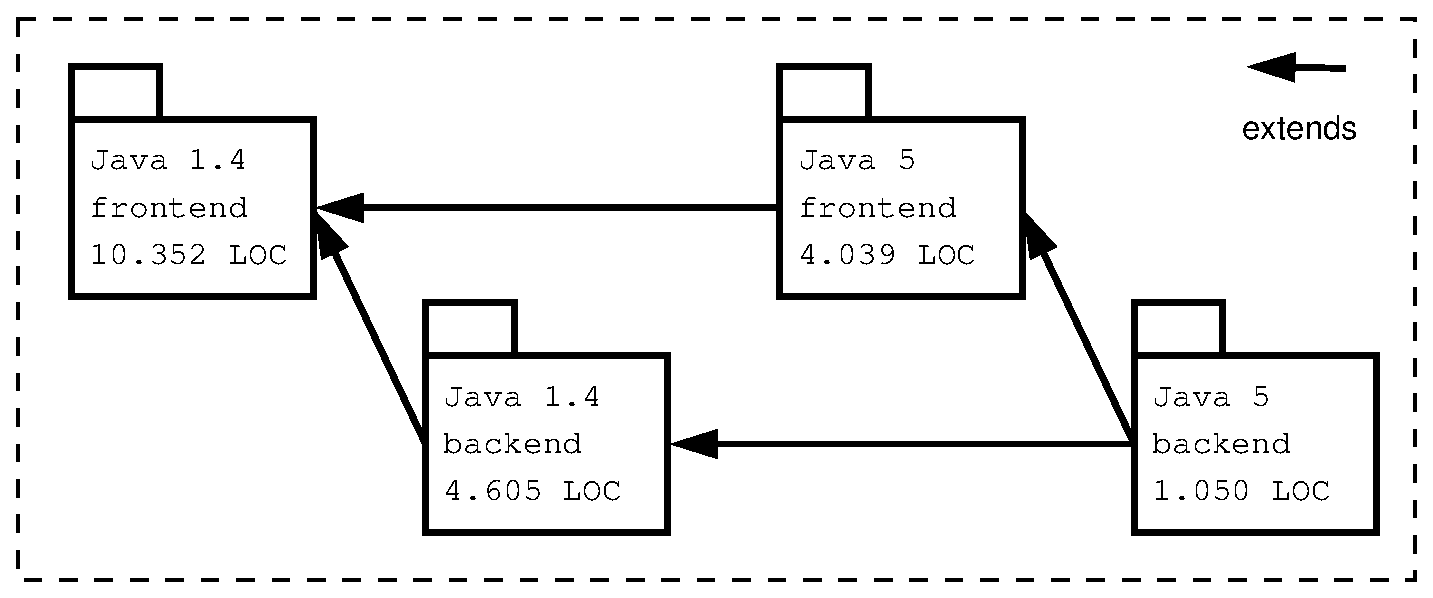
\includegraphics{figures/MainComponents}
    }
    \caption{The main components of JastAddJ}
    \label{MainComponents}
  \end{center}
\end{figure}

The components themselves are composed of AST "`base"' classes, and the
aspects that introduce the ITDs to the said classes. The AST classes
directly or indirectly extend the classes \texttt{ASTNode}, \texttt{List}, and \texttt{Opt},
which form the JastAdd framework classes. 

Since there is no module system each component is represented as a
directory of reusable source files that are combined using build files. The
Java 5 frontend is an extension to the Java 1.4 frontend, reusing its
source file, while specifying Java 5 language features as an increment to
the Java 1.4 frontend. A build file to create a Java 1.4 semantic checker
will thus only include files from the Java 1.4 folder, while a build file
for a Java 5 semantic checker includes files from both folders. The
backends are extensions to the frontends and reuse source files in a
similar manner.  By changing which files to include in the build it is
possible to build four different tools from these components.

Each frontend can be further divided into the following subcomponents: a
parser that builds an AST, a bytecode reader that reads class files, and a
semantic analyzer or code generator. The parser is generated from a context
free grammar, the bytecode reader is written in plain Java, and the
analyzers and code generators are implemented using attribute grammars and
inter-type declarations.

The architecture has a few problems that can be elegantly solved using a
module system. First, the different variants of the compiler can not
coexist in the same system since ITDs destructively update the class
hierarchy. This is handled with an ugly hack where multiple build files and
scripts are used generate compilers to different packages.  Second, the
bytecode readers are implemented in plain Java in a fashion which
unfortunately makes them quite hard to extend and we therefore use
different implementations of the reader in the Java 1.4 frontend and the
Java 5 frontend. This is handled by including different versions of source
files in the build for the Java 5 frontend and excluding some of the files
in the Java 1.4 frontend. Third, the systems are composed into one global
namespace which is terrible from an information hiding point of view.

\subsection{Applying Modules}

To remedy the problems detailed above, we apply the module system to
the JastAddJ compiler. Figure \ref{ModuleMainComponents} shows the basic
architecture of JastAddJ with modules. We have refactored the components such that:

\begin{enumerate}
\item {The JastAdd framework classes reside in their own module.}
\item {The AST classes in the frontend components have been separated from the aspects, and extend the JastAdd framework module.}
\item {The Java 1.5 frontend extends the 1.4 frontend, and similarly with the backends and the AST modules}
\item {Dependencies between the modules were explicitly defined by the use of imports in the module declarations.}
	
\end{enumerate}

\begin{figure}[htb!]
  \begin{center}
    \resizebox{3.2in}{!}{
      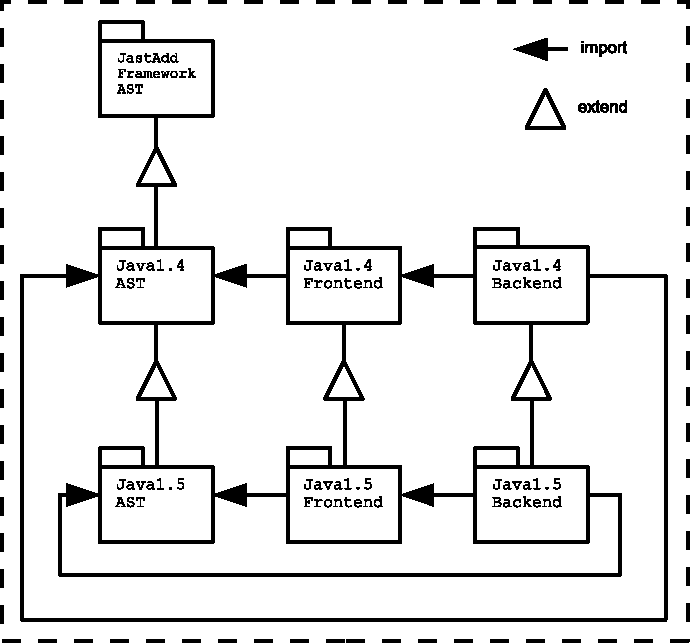
\includegraphics{figures/ModuleMainComponents}
    }
    \caption{JastAddJ refactored to use modules}
    \label{ModuleMainComponents}
  \end{center}
\end{figure}

Other than the necessary changes to use modules, it was also necessary to change the 
access modifiers of several ITDs from package private to public, to allow the 
access of these ITDs from outside their module. 

An example compiler application that uses JastAddJ with modules is shown in the example below.
The module for the compiler application imports a frontend and a backend, and since the backend 
also imports an instance of the frontend, the \texttt{javacompiler} module contains a merge
operation that allows the java compiler and the backend to share the frontend classes.

\begin{lstlisting}[caption={JastAddJ Compiler Application}]
//file javacompiler.module
module javacompiler;
import own java15frontend as frontend;
import own java15backend as backend;
//merge the frontends to point to the same instance
merge frontend, backend::frontend as java15frontend frontend;
\end{lstlisting}

\subsection{Evaluation}

%Shows dependencies explicitly, information hiding, enables sharing through merge
The addition of modules to JastAddJ has made the dependencies of the components
explicit, and will lessen the chance of inadvertently introducing dependencies 
in the future. 

%everything used to be globally visible
%  modules improves information hiding 
%    (concrete example would be nice)
%    percent that became non-global
Information hiding among the components of the system has also benefited from
the introduction of modules. In the previous system, the class files produced from
compilation all belong to the same package, which means that a package private access modifier
is equivalent to a public modifier. Though several ITDs needed to be changed from 
package private to public to allow access from outside, a great majority remained private to
the module. As an example, in the Java 1.4 frontend, 24 ITDs (including synthesized attributes)
were changed from package private to public to allow other modules to access them. This is a small number 
compared to the total number of synthesized attributes alone (541) that were package private in the pre-module version.
This has effectively reduced the public ITD signature of the the Java 1.4 frontend to 5\% of its previous state.

%enables variants with different sets of ITDs
%  examples
The module system also allows instances of the frontend and backend with different versions
to exist in the same system, albeit being unable to share types. This will prove to be useful
in an IDE application, where multiple versions of the frontend would be necessary to provide
as-you-type error checking to different source versions. The ability to instantiate the frontend
without also pulling in the backend will also reduce the size of the AST objects created, as the
ITDs introduced by the backend would not be present in the AST nodes of that instance.

%enables variants with replaced/overridden classes
%  example: bytecode reader
%  (reason, monolithic implementation not suitable for extension, therefore
%  replacement easier)
The use of aspect overriding has allowed the Java 1.5 bytecode parser aspects in the Java 1.5 frontend to
override the corresponding aspects in the Java 1.4 frontend without the build file hacks that involved
excluding the Java 1.4 bytecode parser files when building the 1.5 compiler. This demonstrates that
aspect overriding solves a problem that arises in a real aspect oriented system, as opposed to 
hypothetical examples.


%can we characterize the typical changes needed?
%how intrusive/global were the changes?
The changes required to introduce modules into JastAddJ were minimal: just the addition of the module 
declarations in \texttt{.module} files, the module membership specifications in the existing compilation units,
and a change to the access modifiers of some ITDs to allow inter-module access. Given the benefits of instantiation, 
module composition and information hiding, this is a relatively small price to pay.

%eliminate cycles as a side-effect
%  required by the module system
%  architecture improved/ should have been done that way from the beginning
%  in retrospect
The use of \textbf{own} module instances will also benefit the architecture of JastAddJ,
since cyclic dependencies that involve \textbf{own} instances will cause an error to
be raised by the compiler. This provides a compile-time architecture check to avoid cyclic dependencies,
and would allow the early detection of decisions that would have caused unnecessarily
tight coupling between the components.

%many properties
%are global even though a more local scope would improve information hiding.

%improve extensibility and information hiding



 
 


\section{Implementation}
\label{section:implementation}
We have implemented the module system as an extension to the JastAdd
compiler which adds support for ITDs and attribute grammars as an extension
to the JastAddJ compiler presented in Section~\ref{jastaddjoverview}. 
The extension adds concrete and abstract syntax to support module
specifications and updates name binding and code generation to handle the
new scope and visibility rules imposed by the module system. 

In our previous work we have presented a design how to implement name
binding in a modular extensible fashion, for instance to support new
language features such as inter-type declarations
\cite{jastaddjavacompiler}. It is interesting to note that the same
strategy can be conveniently used to handle name lookup for the presented
module extension. Each module provides lookup for its contained classes and
acts as filter that limits visibility and mangles names. This allowed us to
implement the module system as a completely modular extension that can be
composed with JastAdd much in the same way as the Java 5 compiler extends
the Java 1.4 compiler in Section~\ref{jastaddjoverview}.

The approach is a compile-time based solution where new packages are
generated when multiple instances of the same module is needed, e.g., when
adding different sets of ITDs to the same class hierarchy. Potential name
clashes due to the changed visibility rules are handled by a name mangling
scheme where module names are included in signatures to create unique method
names.

The source is available for download at the following web
site: \texttt{http://builds.jastadd.org/modules}


\section{Related Work}
\label{section:related}
The module system presented in this paper is an aspect-oriented extension of the module
system presented in \textit{Modules as Object-Oriented Types} \cite{modulesastypes}. It
provides the module instantiation, import and merge features that have been described in
this paper. The module instantiation concept was itself was first proposed in iJAM \cite{iJAM}, 
another module system proposed for Java.

The JastAdd compiler framework and the Java compiler \cite{jastadd, jastaddjavacompiler}
was used to implement the system, as well as providing the case study that demonstrated 
the advantages of the module system in terms of information hiding.

Open modules \cite{openmodules, openmodulesaj} has demonstrated that global scope for advice
has detrimental effects on information hiding, and can be solved by
the introduction of a module system that limited the extent of an aspect's effects. The
current module system is based on this philosophy, but has moved the specification of
the module's interface to the components themselves, in the form of access modifiers.
However, access control similar to open modules is still available in the form of the
\textbf{export package} declaration.

Classboxes \cite{classboxj} is a module system for Java that allows the refinement of classes
with mixins within the scope of a classbox, basically a module that is a collection of classes. 
It allows both the base and refined versions to coexist in a single system, even allowing
dispatch of either the base or refined ITD depending on the dynamic type of an object, which
the module system in this paper cannot do. However, classboxes does not address the issue of
module refinement and replacement, which is handled by the extend and merge features of
this paper's module system.

Expanders \cite{expanders} provide functionality similar to ITDs, but allows for finer control
by specifying which ITDs are to be applied to a class in a given context. This provides scope
to an ITD and aids information hiding. However, it does not address the issue of refinement of 
the ITDs themselves.

AspectJ \cite{overviewaspectj}, the current de-facto benchmark for aspect-oriented languages, 
provides ITD refinement through precedence and aspect subtyping. However, these methods are
global in scope, and as has already been discussed previously, does not allow for multiple
versions of the ITD to co-exist in the same system.

CaesarJ\cite{caesarj} is an aspect-oriented language that allows for fine-grained deployment
of aspects, as well as class and aspect refinement through virtual classes\cite{virtualclasses89}. 
The module system in this paper uses an aspect refinement that is similar to virtual classes, but
at the level of the module, instead of the enclosing class. Coupled with the module imports,
we believe that this gives a better extension and composition mechanism for aspect-oriented systems.

Several aspect-oriented languages have allowed for refinement of aspects and ITDs. 
Aspectual mixin layers \cite{aspectualmixinlayers} describes an integration of features from
feature-oriented programming \cite{fopstepwiserefinement} and aspects, and provides a method of 
aspect refinement. However, it does not address the issue of allowing multiple versions of the refined and unrefined 
Aspectual collaborations \cite{lieberherr03aspectual} provides a module-based method for
aspect composition through aspect maps, but again does not address the issue of multiple
ITD versions.

Hyper/J \cite{hyperj} provides the merge operator for the composition of hyperslices, and was
the inspiration behind the merge operation described in this paper. Hyperj's merge, however, addresses
the issue of mixin composition, and not module instance sharing, which is the rationale for
the merge operation in this paper.

%XPIs (in case interfaces come up) \cite{xpi}



\section{Conclusions}
\label{section:conclusions}
We have presented a module system that improves extensibility and
information hiding when using ITDs. Instantiation enables multiple
variants of a base system, each with its own set of applied ITDs. Imports
and exports enable better support for access control improving information
hiding. An important consequence of these features is that they remove some
deficiencies of using plain ITDs compared to a visitor based solution.

The module system has been implemented as an extension to the JastAdd
system, an aspect-oriented attribute grammar extension to Java, which
supports ITDs as one of its major modularization mechanisms. The solution
is purely compile-time and generates class files that can be executed on
a traditional JVM without explicit support for modules.

To evaluate the module system on a realistic system we retrofitted the
JastAdd Extensible Java Compiler (JastAddJ) to use modules. It is a medium
sized application of more than 21.000 lines of code which is designed using
the somewhat extreme viewpoint that the class hierarchy does not contain
any behavior but modularly added using ITDs. Minor changes to the
implementation enabled us to create a family of compilers that can coexist
in the same system using modules compared to the previous solution using an
ugly build file hack. Moreover, it enabled us to limit the scope of many
properties that were global in the original implementation.

As future work we will experiment with using the module instantiation
features to further enhance the reuse of ITDs. One can for instance
envision a situation where ITDs are multiply instantiated in different
modules of the same compiler rather than only across tool boundaries.


%ACKNOWLEDGMENTS are optional
%\section{Acknowledgements}
%\label{section:acknowledgements}
%These are the acknowledgements.

%
% The following two commands are all you need in the
% initial runs of your .tex file to
% produce the bibliography for the citations in your paper.
\bibliographystyle{abbrv}
\bibliography{sigproc}  % sigproc.bib is the name of the Bibliography in this case
% You must have a proper ".bib" file
%  and remember to run:
% latex bibtex latex latex
% to resolve all references
%
% ACM needs 'a single self-contained file'!
%
\end{document}
